\section{ХОД РАБОТЫ}

\subsection{Задание}

Необходимо решить задачу повышения производительности труда не ниже заданного уровня
при соблюдении установленного лимита капитальных вложений. В соответствии с первым вариантом
имеем следующие исходные данные:

\begin{itemize}
  \item планируемый прирост производительности труда за год ---~8,0~\%;
  \item сумма выделенных капитальных вложений ---~355~млн~ден.~ед.;
  \item общая численность промышленно-производственного персонала ---~2200~чел.
\end{itemize}

\subsection{Решение задачи}

\paragraph{Подбор мероприятий.}

Необходимо подобрать мероприятия, обеспечивающие плановый прирост производительности
труда, в пределах выделенного лимита капитальных вложений. Для облегчения процесса
подбора мероприятий выполним следующие действия:

\begin{itemize}
  \item для каждого мероприятия рассчитаем <<эффективность применения>>,
    как годовое повышение производительности труда, разделенное на капитальные вложения;
  \item отсортируем мероприятия по <<эффективности применения>>.
\end{itemize}

На рисунках~\ref{fig:tabl12}~--~\ref{fig:tabl14} представлены результаты проделанных операций.

\begin{figure}[htbp]
  \centering
  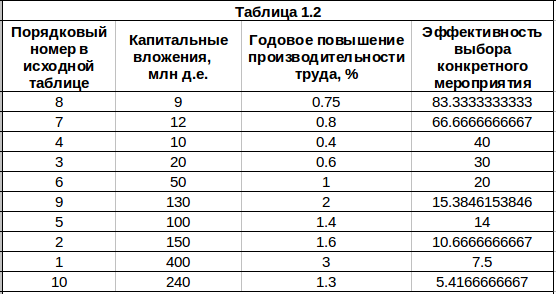
\includegraphics[width=0.8\linewidth]{img/tabl12}
  \caption{Таблица~1.2 после сортировки}\label{fig:tabl12}
\end{figure}

\begin{figure}[htbp]
  \centering
  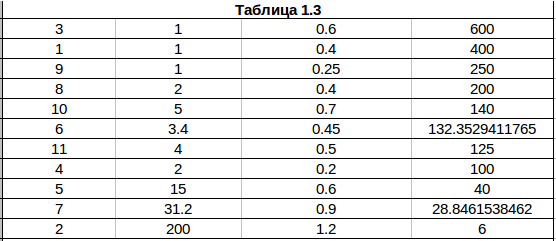
\includegraphics[width=0.8\linewidth]{img/tabl13}
  \caption{Таблица~1.3 после сортировки}\label{fig:tabl13}
\end{figure}

\begin{figure}[htbp]
  \centering
  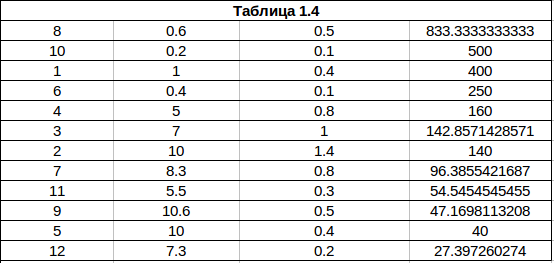
\includegraphics[width=0.8\linewidth]{img/tabl14}
  \caption{Таблица~1.4 после сортировки}\label{fig:tabl14}
\end{figure}

\newpage

Далее будем выбирать мероприятия с высокой <<эффективностью>> --- так, чтобы планируемый
прирост производительности труда составил 8\%. Список выбранных мероприятий
представлен в таблице~\ref{tbl:solution}.

\begin{table}[htbp]
  \caption{Выбранные мероприятия\label{tbl:solution}}
  \centering
    \begin{tabular}{| m{3cm} | m{3cm} | m{3.5cm} | m{4.5cm} |}
      \hline
      Таблица-источник мероприятия & Порядковый номер \newline в таблице & Капитальные \newline вложения, млн~ден.~ед. & Повышение \newline производительности труда, \% \\ \hline
      1.2 & 7 & 12 & 0.8 \\ \hline
      1.2 & 8 & 9 & 0.75 \\ \hline
      \multicolumn{2}{|l|}{Итого по \textbf{I} группе:} & \textbf{21} & \textbf{1.55} \\ \hline
      1.3 & 1 & 1 & 0.4 \\ \hline
      1.3 & 3 & 1 & 0.6 \\ \hline
      1.3 & 5 & 15 & 0.6 \\ \hline
      1.3 & 8 & 2 & 0.4 \\ \hline
      1.3 & 9 & 1 & 0.25 \\ \hline
      1.3 & 10 & 5 & 0.7 \\ \hline
      \multicolumn{2}{|l|}{Итого по \textbf{II} группе:} & \textbf{25} & \textbf{2.95} \\ \hline
      1.4 & 1 & 1 & 0.4 \\ \hline
      1.4 & 3 & 7 & 1 \\ \hline
      1.4 & 4 & 5 & 0.8 \\ \hline
      1.4 & 7 & 8.3 & 0.8 \\ \hline
      1.4 & 8 & 0.6 & 0.5 \\ \hline
      \multicolumn{2}{|l|}{Итого по \textbf{III} группе:} & \textbf{21.9} & \textbf{3.5} \\ \hline
      \multicolumn{2}{|l|}{Итого:} & 67.9 & 8 \\ \hline
    \end{tabular}
\end{table}

\paragraph{Расчет абсолютной экономии численности промышленно-производственного
 персонала} производится по формуле:
\begin{equation}
\% ~ \text{ПП} = \dfrac{\text{Ч}}{\text{Ч}_{\text{ПЛ}} - \text{Ч}} \cdot 100
\end{equation}

Выразим из этой формулы Ч. В итоге:
\begin{equation}
\text{Ч} = \dfrac{\% ~ \text{ПП} \cdot \text{Ч}_{\text{ПЛ}}}{100 + \% ~ \text{ПП}}
\end{equation}

Вычислим Ч по каждой группе мероприятий.
\begin{align}
  \text{Ч}_{I} = \dfrac{1.55 \cdot 2200}{100 + 1.55} = 33 ~ \text{чел.} \\
  \text{Ч}_{II} = \dfrac{2.95 \cdot 2200}{100 + 2.95} = 63 ~ \text{чел.} \\
  \text{Ч}_{III} = \dfrac{3.5 \cdot 2200}{100 + 3.5} = 74 ~ \text{чел.}
\end{align}

Итого за счет проведённых мероприятий абсолютная экономия численности
промышленно-производственного персонала составила \textbf{170 человек.}

\newpage
